\documentclass [a4paper, 11pt]{article}

\usepackage{amssymb}
\usepackage{epsfig}
\usepackage{graphicx}
\usepackage{times}
\usepackage{float}
\usepackage[usenames,dvipsnames]{color}
\usepackage{scrlayer-scrpage}
\pagestyle{scrheadings}
\clearpairofpagestyles
\usepackage{hyperref}
\usepackage{amsmath}
\usepackage{latexsym}
\usepackage[font=small,labelfont=bf,figurename=Figure]{caption}                                                                                   
\usepackage[font=small,labelfont=bf]{subcaption}
\usepackage{nicefrac}
\usepackage{mathtools}
\usepackage{pgfgantt}
\usepackage{wrapfig}
\usepackage{graphics}
\usepackage[wide,ragged]{sidecap}
\usepackage{todonotes}
\usepackage{enumitem} % BK to change itemize margins
\usepackage[utf8]{inputenc}
\usepackage{placeins}
\usepackage{mathbbol}
\usepackage[noabbrev,capitalise]{cleveref}
\usepackage{tabularx}
\usepackage{cite}
\usepackage{booktabs}
%%% \usepackage{longtable}
%%% \usepackage{multirow}
\usepackage{wrapfig}
\usepackage{tabu}
\usepackage{threeparttable}
\usepackage{threeparttablex}
\usepackage{makecell}
\usepackage{braket}
\usepackage{color, colortbl}
\usepackage[compat=1.0.0]{tikz-feynman}
\usepackage{bm}      % for \bm macro 
\definecolor{Gray}{gray}{0.8}


\newcommand{\be}{\begin{equation}}
\newcommand{\ee}{\end{equation}}
\newcommand{\bea}{\begin{eqnarray}}
\newcommand{\eea}{\end{eqnarray}}
\newcommand{\nn}{\nonumber}
\newcommand{\lsim}{\mathop{\lsi}}
\newcommand{\gsim}{\mathop{\gsi}}

\def\fm{\,{\rm fm}}
\newcommand{\Oa}{{\rm O}(a)}

\newcommand{\dtau}{\Delta\hspace{-.06cm}\tau}
\newcommand{\tr}{\operatorname{Tr}}
\newcommand{\re}{\operatorname{Re}}
\newcommand{\im}{\operatorname{Im}}


\definecolor{sand}{RGB}{234,185,12}
\def\slash#1{\mbox{$\not\!\! #1$}}
\def\Dslash{{\slash D}}
\newcommand{\<}{\langle}
\renewcommand{\>}{\rangle}
\newcommand{\la}{\langle}
\newcommand{\ra}{\rangle}
\newcommand{\beq}{\begin{equation}}
\newcommand{\eeq}{\end{equation}}
\newcommand{\beqn}{\begin{eqnarray}}
\newcommand{\eeqn}{\end{eqnarray}}
\newcommand{\wt}{\widetilde}
\newcommand{\idnty}{\hbox{1$\!\!$1}}
\newcommand{\vettq}{\mbox{\bf{q}}}
\newcommand{\vettx}{\mbox{\bf{x}}}
\newcommand{\Li}{{\cal L}}
\newcommand{\bfr}{{\bf r}}
\newcommand{\bfp}{{\bf p}}
\newcommand{\half}{\frac{1}{2}}
\newcommand{\pslash}{\not\hspace{-3pt}p}
\newcommand{\mev}{\,\mathrm{MeV}}
\newcommand{\gev}{\,\mathrm{GeV}}
\newcommand{\fermi}{\,\mathrm{fm}}
\newcommand{\brackets}[1]{\langle #1 \rangle}
\newcommand{\Oop}{\mathcal{O}}
%\newcommand{\pvec}{\vec{p}}
%\newcommand{\Pvec}{\vec{P}}
%\newcommand{\xvec}{\vec{x}}
\newcommand{\DDalphaAMG}{\mathrm{DD}\alpha\mathrm{AMG}}
\newcommand{\Pvec}{\mathbf{P}}
\newcommand{\pvec}{\mathbf{p}}
\newcommand{\qvec}{\mathbf{q}}
\newcommand{\dvec}{\mathbf{d}}
\newcommand{\xvec}{\mathbf{x}}
\newcommand{\yvec}{\mathbf{y}}
\newcommand{\zvec}{\mathbf{z}}
\newcommand{\epow}[1]{\mathrm{e}^{#1}}

\newcommand{\projectA}{Study of excited energy levels in three-pion scattering}
\newcommand{\projectB}{Large time extent simulation for scattering processes}

\newcommand{\amulohvp}{a_{\mu}^{\mathrm{LO-HVP}}}

\newcommand{\psibar}{\bar{\psi}}
\newcommand{\ubar}{\bar{u}}
\newcommand{\dbar}{\bar{d}}
\newcommand{\sbar}{\bar{s}}
\newcommand{\cbar}{\bar{c}}
\newcommand{\Dcovlr}{\overset{\leftrightarrow}{D}}
\newcommand{\Dcovmulr}{\overset{\leftrightarrow}{D^\mu}}
\newcommand{\Dcovnulr}{\overset{\leftrightarrow}{D^\nu}}
\newcommand{\avgx}{\brackets{x}}
\newcommand{\gammafive}{\gamma_5}
\newcommand{\qbar}{\bar q}
\newcommand{\order}[1]{\mathcal{O}({#1})}

\textwidth 16 cm
\textheight 23 cm
\setlength{\oddsidemargin}{0.1 cm}
\setlength{\topmargin}{1 cm}
\setlength{\headheight}{0cm}
\setlength{\headsep}{0cm}
\setlength{\footskip}{0.75cm}
\setlength{\parindent}{0cm}
\setlength{\oddsidemargin}{0.1 cm}
\setlength{\itemsep}{10pt}
\bibliographystyle{gcs}
\cfoot{\pagemark}
\ofoot{\tiny V1.8-2020DEC02}
 
\begin{document}
 
\begin{figure}[H]
\begin{center}
  
\includegraphics[scale=0.45]{Figures/GCS-hlrs-fzj-lrz.jpg}\\
\end{center}
\end{figure}

\begin{center}
{\LARGE \bf Project Proposal for Tier 0/Tier 1 HPC Access} \\

\bigskip
\bigskip
\bigskip
\end{center}
\textbf{Period}\\
\phantom{MM}\textit{10.2024-9.2025}

\bigskip
\textbf{Project title}\\
\phantom{MM}\textit{Inclusive semileptonic decay rates from lattice QCD}

\bigskip
\textbf{Type of project}\\
\phantom{MM} continuation

\bigskip
\textbf{HPC system(s) and corresponding centre(s)}\\
\phantom{MM} \textit{JUWELS Booster, JSC}

\bigskip
\textbf{Project ID or project acronym}\\
\phantom{MM} \textit{ISDLQCD}%\textit{Please provide in case of a project extension}

\bigskip
\textbf{Principal investigator}\\
\phantom{MM} \textit{C. Urbach, Helmholtz-Institut für Strahlen- und Kernphysik (Theorie) and
	Bethe Center for Theoretical Physics, University of Bonn, 53115 Bonn, Germany}

\bigskip
\textbf{Project contributor(s)}\\
\phantom{MM} \textit{ 
 A.~Evangelista$^a$,
 R.~Frezzotti$^a$,
 G.~Gagliardi$^b$,
 M.~Garofalo$^c$,
 C.~Groß$^c$,
 B.~Kostrzewa$^d$,
 V.~Lubicz$^e$,
 M.~Panero$^f$,
 F.~Sanfilippo$^b$,
 S.~Simula$^b$,
 A~Smecca$^g$,
 N.~Tantalo$^a$
}\\ 

\textit{$^a$ Dipartimento di Fisica and INFN, Universit\`a di Roma ``Tor Vergata", Via della Ricerca Scientifica 1, I-00133 Roma, Italy}\\
\textit{$^b$ Instituto Nazionale di Fisica Nucleare, Sezione di Roma Tre, Via della Vasca Navale 84, I-00146 Rome, Italy }\\
\textit{$^c$ Helmholtz-Institut f{\"u}r Strahlen- und Kernphysik (Theorie) and Bethe Center for Theoretical Physics, Universit{\"a}t Bonn}\\
\textit{$^d$ High Performance Computing and Analytics Lab, University of Bonn, 53115 Bonn, Germany} \\
\textit{$^e$ Dipartimento di Matematica e Fisica, Universit\`a Roma Tre and INFN, Sezione di Roma Tre, Via della Vasca Navale 84, I-00146 Rome, Italy} \\
\textit{$^f$ Dipartimento di Fisica, Università di Torino \& INFN, Sezione di Torino, Via Pietro Giuria 1, I-10125 Turin, Italy}\\
\textit{$^g$ Department of Physics, Faculty of Science and Engineering, Swansea University (Singleton Park Campus) Singleton Park, SA2 8PP Swansea, Wales, United Kingdom}
\vfill

\newpage

\vfill
\tableofcontents
\vfill

\newpage

\section{Introduction}

\rule{\textwidth}{0.4pt}

In many precision tests of the Standard Model (SM) of Particle Physics and
searches for New Physics beyond it, a precise understanding of hadron
structure and interactions is needed to provide ab initio predictions
to be compared with experimental data. The fundamental forces of Quantum
Chromodynamics (QCD) at low energy describe particles, namely mesons and
baryons, as the non-perturbative realisation of confined quarks interacting
via gluons. The only rigorous treatment of such non-perturbative
dynamics known to date is based on the regularisation of the theory on
a finite, discrete Euclidean space-time lattice, and subsequent
numerical simulations of the discretised theory. This allows one to
compute hadronic matrix elements of great phenomenological interest,
such as e.g those regulating hadron structure and fragmentation, decays and transition
amplitudes among different flavours of hadrons, and hadronic corrections
to electroweak precision observables.
%affecting precision observables, among others.

Flavour physics is currently one of the fields with a high potential
for the discovery of a statistically significant discrepancy between the SM and
experiment. Among others, there could be additional flavour-changing
interactions, further complex phases in the Cabibbo-Kobayashi-Maskawa (CKM)
matrix, or possible violations
of lepton-flavour universality. Even if the mass scales of new
particles beyond the SM turned out to be very high, quantum effects of
the associated fields could leave detectable imprints on the physics
of heavy quarks.
This makes precise theoretical computations of related observables
highly desirable. In particular, semi-leptonic decays of heavy mesons
and elements of the CKM matrix are very
interesting to estimate accurately from first principles.

Until recently, most lattice calculations focused on the investigation
of exclusive decays because inclusive processes consist
of a potentially very large number of physical states and their
systematic analysis in lattice QCD calculations was impractical.
However, novel approaches have been put forward that allow one to address
inclusive decays in lattice QCD, like the method described in
Ref.~\cite{Gambino:2020crt} where the total decay rate for the process
$D_s \to X\ell\bar\nu$ and $B \to X\ell\bar\nu$   is related to a smeared spectral
density that can be computed from an Euclidean four-point function in a finite
volume~\cite{Hansen:2019idp} (see
also \cite{Bulava:2019kbi,Bulava:2021fre,Gambino:2022dvu}). The computation of such
Euclidean correlation functions is standard and can be carried out
with high precision.
The reconstruction of the spectral densities
represents the main challenge that was already carried out for the $D_s$ meson
in the previous computer time allocation of this project and the results were
presented at the $41^{\mbox{st}}$ Lattice Conference at the University of Liverpool
\cite{talklatt2024_ale, talklatt2024_chr}
and a paper is in preparation.

With this continuation of the computer time application, we propose to extend
the calculation of the total decay rate for the process $D_s \to X\ell\bar\nu$ to the
heavier $B$ and $B_s$ meson computing  $B (B_s) \to X\ell\bar\nu$.
As in the previous time contingent we are including the continuum limit
using the $N_f=2+1+1$ clover twisted-mass action with physical
values of up/down, strange and charm
quarks~\cite{ExtendedTwistedMass:2021qui,ExtendedTwistedMass:2021gbo,ExtendedTwistedMass:2022jpw}.
A necessary preliminary step to compute the inclusive decay rate of the $B_s$
meson is the determination of the
$B$ physical point, i.e. the value of the bare parameter of the $b$-quark mass that reproduces the
experimental value of the $B$-meson mass.
% quark bottom mass $m_b$.
This can be
achieved using the ratio method proposed in \cite{ETM:2009sed}
and successfully used in \cite{ETM:2016nbo}, where suitable ratios allow
to reach the bottom quark sector by combining simulations around the
charm-quark mass with an exactly known static limit.
The bare quark mass can then be converted in to renormilized values my multiply
the appropriate renormalization constant $Z_p$ which computation by the ETMC
is under finalization.


% The continuation of the project to the $B_s$ meson is very interesting from the
% experimental side  where recent results from $B$ factories reveal some tension with
% SM predictions, but also exhibit puzzling discrepancies between exclusive and
% inclusive channels~\cite{ParticleDataGroup:2020ssz, HFLAV:2019otj, Gambino:2019sif}
% {\color{red} is there an update??}
The continuation of the project, aiming at the computation of the $B_{(s)}\to X \ell\nu$
inclusive decay rates, is very interesting and potentially very important from
the phenomenological perspective. Indeed, recent results from $B$ factories reveal
some tension with SM predictions and, moreover, confirm the long-standing puzzling
discrepancies between exclusive and inclusive deteminations of the $V_{cb}$ and
$V_{ub}$ CKM matrix elements~\cite{ParticleDataGroup:2022pth, HFLAV:2022esi, Gambino:2019sif}.
%The theoretical study of semileptonic decays of heavy mesons encode direct information on the modulus of the elements of the
%Cabibbo-Kobayashi-Maskawa (CKM) quark mixing matrix \cite{Cabibbo:1963yz, Kobayashi:1973fv}. 
%By using the optical theorem, the total inclusive decay rate for the process $D_s \to X\ell\bar\nu$ can be written
%$|V_{cd}|$, $|V_{cs}|$ and $|V_{us}|$
%\begin{equation}
%	\Gamma = G^2_F\left\{ |V_{cd} |^2 \Gamma_{cd} + |V_{cs} |^2 \Gamma_{cs} + |V_{us} |^2 \Gamma_{su}
%	\right\}\,,
%\end{equation}



\section{Preliminary Work}
\rule{\textwidth}{0.4pt} 


The proposed project aims to continue GCS Large Scale projec ISDLQCD
(application number 28958) and the long term activities of the
Extended Twisted Mass Collaboration (ETMC) in the calculation of
hadronic matrix elements via lattice QCD simulations. ETMC has
produced and is still producing gauge configuration ensembles at
different lattice spacing values at the physical point, by which we
mean physical values of all the dynamical quark masses. For the
proposal here we propose to use four values of the lattice spacing,
corresponding to the ensembles compiled in Table~\ref{tab:ensembles}. The
ensembles labelled with $B$, $C$, $D$, $E$ have been produced already
and used in several ETMC
works~\cite{ExtendedTwistedMass:2021qui,ExtendedTwistedMass:2021gbo,ExtendedTwistedMass:2022jpw,ExtendedTwistedMassCollaborationETMC:2022sta}
an in the previous stage of this project.
These four lattice spacing values will enable a controlled continuum
limit of the quantities relevant to this proposal.
Moreover, at the $B$ value of the lattice spacing we have
three volumes available, which will allow us to check finite volume
effects representing a main source of systematic uncertainty.
Since we work directly at physical light quark mass values, no
extrapolation in the light quark mass values is necessary.

For the continuum limit we additionally benefit from automatic
$\mathcal{O}(a)$-improvement of the physical observables in question
thanks to the twisted mass action at
maximal twist, ensuring convergence to the continuum
limit with scaling violations of order $a^2$~\cite{Frezzotti:2003ni}.

\begin{SCtable}[.4]
	\centering % center the table
	\begin{tabular}{lccccr} % alignment of each column data
		\toprule
		name          & $L$ [fm]      & $a$
		[fm]          & $M_\pi$ [MeV] & $M_\pi L$                         \\
		\midrule
		% cAp211.077.64 & 5.76 & $\sim$0.09 & $\approx$ 135 & 3.95  \\
		\midrule
		cB211.072.48  & 3.84          & $\sim$0.08 & $\approx$ 135 & 2.63 \\
		cB211.072.64  & 5.12          & $\sim$0.08 & $\approx$ 135 & 3.51 \\
		cB211.072.96  & 7.68          & $\sim$0.08 & $\approx$ 135 & 5.27 \\
		\hline
		cC211.06.80   & 5.44          & $\sim$0.07 & $\approx$ 135 & 3.72 \\
		% cC211.06.112  & 7.62          & $\sim$0.07 & $\approx$ 135 & 5.21 \\
		\hline
		cD211.054.96  & 5.76          & $\sim$0.06 & $\approx$ 135 & 3.94 \\
		\hline
		cE211.044.112 & 5.48          & $\sim$0.05 & $\approx$ 135 & 3.75 \\
		\bottomrule
	\end{tabular}
	\caption{ETMC's $N_f=2+1+1$ gauge ensembles relevant for this
		proposal. The time extent is always set to $T=2L$.}
	\label{tab:ensembles}
\end{SCtable}

% In addition to the feasibility study presented by the authors of
% Ref.~\cite{Gambino:2022dvu} including some of the project contributors of this
% project, we have performed a first exploratory investigation of
% charm-down quark part of the
% differential decay rate of the $D_s$ meson decaying into $X\ell\nu$ on
% the cB211.072.64 ensemble, for the first time at the physical
% point. The result is shown in Figure~\ref{fig:Gamma_B64}.

The computation of the bottom quark mass was already performed with
the previous generation of gauge ensembles of ETMC~\cite{ETM:2016nbo,ETM:2011zey} with
non physical pion masses, smaller volumes and coarser lattice spacing.
With the most recent ensambles of ETMC some B physics has been studied, by some outhors
that are present in this application, in \cite{Frezzotti:2024kqk}
but an hadronic scheme was used to determine the physical $B$ meson point, here we propose to 
determine the renormalized bottom quark mass.   


The computation of the   inclusive decay rate we are finalizing the
analysis of the $D_s\to X \ell \nu$ Figure~\ref{fig:dGammadq_Ds} and
we will use an extrapolation guided by heavy quark effective theory to extrapolate
to the $b$ quark mass.
From  Figure~\ref{fig:dGammadq_Ds} we show that the statistical and systematic
uncertainty can be controlled  the
dependence on the squared momentum can be resolved. This makes us
confident that the proposed project is feasible.

\endinput



\section{Description of the Project}
\rule{\textwidth}{0.4pt}
\subsection{Project Details}

\label{sec:proj}

The computation proposed here will use the same ensembles of the previous stage of the project
i.e. Wilson-clover twisted
mass fermions~\cite{Alexandrou:2018egz}. The up/down quarks will be treated
in a fully unitary setting. To avoid flavor mixing lattice artefacts
in the unitary strange/charm sector of this regularisation, we use a
mixed action approach for strange and charm quarks: so-called
Osterwalder-Seiler type~\cite{Frezzotti:2004wz} strange and charm quark doublets
$(s^+ , s^-)^T$ and $(c^+ , c^- )^T$ are added with bare
twisted strange and charm quark mass $\pm \mu_s$ and $\pm \mu_c$
tuned to reproduce the physical mass of the $\phi$ and $J/\Psi$
mesons, respectively, as described in Appendix C of
Ref.\cite{ExtendedTwistedMass:2022jpw}. For more details, we refer to
this reference.


The core of our project is the calculation of inclusive semi-leptonic
decays of the $B$ and $B_s$ mesons, for which we need to determine the
bare $b$-quark mass first.
For the application of what we call the
ratio-method~\cite{ETM:2009sed}, we will generate data at six
different values of the heavy quark mass in the range from 
1 to 3.5 times the charm quark mass. 
The data produced for these six heavy quark mass values can be used at
the same time for the  determination of the $B$ and $B_s$ meson masses
and the total inclusive decay rate for the process $B_{(s)} \to
X\ell\bar\nu$. 



%%%%%%%%%%%%%%%%%%%%%%%%%%%%%%%%%%%%%%%%%%%%%%%%%%%%%%%%%%%%%%%%%%%%%%%%%%%%%%%%%%
%%%%%%%%%%%%%%%%%%%%%%%%%%%%%%%%%%%%%%%%%%%%%%%%%%%%%%%%%%%%%%%%%%%%%%%%%%%%%%%%%%
\subsection{Sub-project 1: total inclusive decay rate $B_s \to X\ell\bar\nu$}

By using the optical theorem, the semi-leptonic decay of a $B$ and $B_s$
to a hadron $X$ with a pair of massless leptons $B_{(s)} \to X\ell\bar\nu$ can be written as
\begin{equation}
  \Gamma = G^2_F\left\{ |V_{bu} |^2 \Gamma_{bu} + |V_{bc} |^2 \Gamma_{bc} + |V_{su} |^2 \Gamma_{su}
  \right\}\,,
  % \Gamma_c = G^2_F |V_{bc} |^2 \Gamma_{bc}\,.
\end{equation}
where the different contributions on the right-hand-side correspond at the quark level
to the weak transitions $b \to u$, $b \to c$ and $s \to u$, respectively.
Each contribution can be written as
\begin{equation}\label{eq:Gamma_fg}
  \Gamma_{fg}=\int \frac{d^3p_\nu}{(2\pi)^32E_\nu}\frac{d^3p_\ell}{(2\pi)^32E_\ell}
  L_{\mu\nu}(p_\ell, p_\nu) H^{\mu\nu}_{fg}(p,p-p_\ell-p_\nu)\,,
\end{equation}
where the leptonic tensor is given by
\begin{equation}
  L_{\mu\nu}(p_\ell, p_\nu) =4\left\{p_\ell^\mu p_\nu^\nu +p_\ell^\nu
  p_\nu^\mu - g^{\mu\nu} p_\ell\cdot p_\nu+
  i\epsilon_{\mu\nu\alpha\beta} p_\ell^\alpha p_\nu^\beta\right\}\,,
\end{equation}
while the hadronic tensor reads
\begin{equation}
  H^{\mu\nu}_{fg}(p,p_X)=\frac{1}{2m_{B_{(s)}}}\langle B_{(s)}| J^\mu_{fg}(0)(2\pi)^4
  \delta^4(\mathbb{P}-p_x) J^{\nu\dagger}_{gf} (0)| B_{(s)}\rangle\,.
\end{equation}
$\mathbb{P}$ is the QCD four momentum operator and $J_{fg}$ are the
relevant Minkowski weak currents $J_{fg}^\mu(x)=i\bar
  f(x)\gamma^\mu(1-\gamma_5)g(x)$.
The contribution $\Gamma_{su}$ is zero in the decay of the $B$ for
momentum conservation while  in the decay of the $B_{s}$ it is
suppressed by the integration over the phase space of
\eqref{eq:Gamma_fg}. Moreover, this flavour channel is only inclusive
through $B_s\to B\ell\bar\nu$. 
The calculation of $\Gamma_{bu}$  requires computing disconnected
diagrams, which is computationally more challenging than the connected
part. 
On the other hand the contribution coming from disconnected diagrams
is expected to be small due to the OZI-suppression rule. 
In this project we will focus only on the computation of $\Gamma_{bc}$
and the connected part of $\Gamma_{bu}$ leaving the computation of the
disconnected diagram to a followup project. 
It is important to notice that the decays $B_{(s)} \to X_c\ell\bar\nu$ corresponding to decays into charmed final states $X_c$ are known from the experimental side and thus can be compared directly with our calculations.

From now on we will drop the indices $fg$
and the procedure we are describing will be equivalent for the $bu$ and $bc$ contributions,
moreover
in the rest frame of the $B_{(s)}$ meson we have $p=(M_{B_{(s)}},\bm{0})$ thus we simplify the notation of
$H^{\mu\nu}(p_X)\equiv H^{\mu\nu}_{fg}(p,p_X)$.
The hadronic tensor $H_{\mu\nu}$ is
the spectral density of the quantity
\begin{equation}
  M_{\mu\nu}(t,{\bf q})= \int_0^{\infty}d \omega H_{\mu\nu} (\omega,{\bf q}) e^{-\omega t}\,,\quad \text{with}\quad p_X=(\omega,\bm{q})\,.
\end{equation}
$H_{\mu\nu}$ can be reconstructed from $M_{\mu\nu}$ using the method presented in
Ref.~\cite{Hansen:2019idp}. $M_{\mu\nu}$ can be directly computed from the
ratio of Euclidean lattice correlators
\begin{gather}
  M_{\mu\nu}(t_2-t_1,{\bf q})=\frac{C_{\mu\nu}(t_{snk},t_2,t_1,t_{src};q)}{e^{-(t_{snk}-t_2)}  C(t_1-t_{src}) }\label{eq:ratio_4pt_2pt}\\
  \label{eq:4pt}
  C_{\mu\nu}(t_{snk},t_2,t_1,t_{src};q)=\int d^3x e^{i{\bf q}\cdot {\bf x}}
  \langle B_{(s)}({\bf 0}, t_{snk}) J^{\dagger}_\mu({\bf x},t_2)  J_\nu(0,t_1)
  B_{(s)}^\dagger({\bf 0}, t_{src})\rangle\,,\\
  \label{eq:2pt}
  C(t_{snk}-t_{src}) =  \langle B_{(s)}({\bf 0}, t_{snk})
  B_{(s)}^\dagger({\bf 0}, t_{src})\rangle\,.
\end{gather}
In general, the inverse problem represented by the extraction of
hadronic spectral densities from Euclidean correlators is notoriously
ill-posed. Recently, a method to cope with these problems has been
proposed in Ref.~\cite{Hansen:2019idp}. It consists of treating the
integrals mentioned above with some $C_\infty$ kernel $K_\sigma$
\begin{equation}
  H^\sigma_{\mu\nu}(\omega^*, {\bf q})= \int d \omega K_\sigma( \omega^*,\omega ) H_{\mu\nu}(\omega, {\bf q})\,,
\end{equation}
making the inverse problem well posed and $H^\sigma_{\mu\nu}$ computable.
In our case the phase space integration in \eqref{eq:Gamma_fg}
provides a sharp smearing kernel function $\theta$. Following
Refs.~\cite{Gambino:2020crt, Gambino:2022dvu}, the phase space integral over
\eqref{eq:Gamma_fg} can be written as
\begin{gather}
  \frac{48 \pi^4}{m_{B_{(s)}}^5}\frac{d\Gamma}{d \bm{ \omega^2} }
  =\sum_{l=0}^2 |\bm{\omega}|^{3-l}\int_0^{\infty}d \omega_0 \Theta^l(\omega_0^{max}-\omega_0) Z^l\,,\quad\quad {\omega}_0^{max}=1-|\bm{\omega}|\,,\quad\Theta^l(x)=x^l\theta(x)\\
  Z^2=Y_3-2Y_1\,,\quad Z^1=2(Y_3-2Y_1-Y_4)\,,\quad Z^0=Y_2+Y_3-2Y_4\,.
\end{gather}
Moreover, the $Y_i$ can be directly computed from the Euclidean
hadronic tensor $H^{\mu\nu}$ as follows
\begin{align}
                                                     & Y^1=-m_{B_{(s)}}\sum_{ij}\hat{n}^i\hat{n}^j H^{ij}(p,q)\,,          &  & Y^2=-m_{B_{(s)}}H^{00}(p,q)\,, \\
                                                     & Y^3=m_{B_{(s)}}\sum_{ij}\hat{\omega}^i\hat{\omega}^j H^{ij}(p,q)\,, &  &
  Y^4=-im_{B_{(s)}}\sum_{i}\hat{\omega}^i H^{0i}(p,q)\,, &
\end{align}
with $\hat{n}$ a unit vector orthogonal to $\bm\omega$.
Thus, the phase space integral provides us a $\theta$-function smearing
kernel. However, the $\theta$-function is not smooth, which is why we
will use a $C_\infty$ kernel that
after taking the infinite volume limit, the
$\theta$-function is recovered as $\sigma\to0$, i.e. $\lim_{\sigma\to 0} K_\sigma^l(x^*,x)=\Theta^l(x^*-x)$.
Therefore,
\begin{gather}
  \frac{48 \pi^4}{m_{B_{(s)}}^5}\frac{d\Gamma}{d \bm{ \omega^2} }
  =\lim_{\sigma\to 0}\sum_{l=0}^2 |\bm{\omega}|^{3-l}\int_0^{\infty}d \omega_0 K_\sigma^l(\omega_0^{max},\omega_0) Z^l\,.
\end{gather}
The spectral reconstruction can be performed at the analysis stage. Thus,
the main cost of this calculation is the production of the
four-point functions \eqref{eq:4pt}.

The renormalization constants necessary to renormalise the ratio of
correlators \eqref{eq:ratio_4pt_2pt} $Z_A$ and $Z_V$ have already been
computed in previous work of ETMC~\cite{ExtendedTwistedMass:2024myu}.

\begin{figure}
  \centering
  \begin{tikzpicture}
    \begin{feynman}[scale=1.5]
      \vertex[anchor=east,blob, fill=black!0!] (a) at (0,0) {\(B_{(s)}^\dagger\)};
      \vertex[anchor=east,blob, fill=black!0!]  (J1) at (1,0.8) {\(J_W\)};
      \vertex[anchor=east,blob, fill=black!0!] (J2) at (2.4,0.8) {\(J_W\)};
      \vertex[anchor=west,blob, fill=black!0!] (b) at (3,0) {\(B_{(s)}\)};
      \vertex (s1) at (3.4,-0.4) ;
      \vertex (s2) at (3.4, 0.4) ;
      \vertex (s3) at (2.6, 0.7) ;
      \vertex (s4) at (1.8, 1) ;

      \diagram*{
      %				(a) --[fermion,  half right,looseness=0.5,edge label=$s$] (b);
      (b) --[fermion, black, out=220, in=320,edge label=$u(s)$,swap] (a);

      (a) --[fermion, blue, edge label=$b$] (J1) ;
      (J1) --[fermion, sand, edge label=$c$, reversed momentum'=$\bf{q}$] (J2);
      (J2) --[fermion, blue ,edge label=$b$] (b);
      (s1) --[->, half right, edge label=sequential,swap] (s2);
      (s3) --[->, half right, edge label=sequential,swap] (s4);
      };
    \end{feynman}
    \begin{feynman}[scale=1.5]
      \vertex[anchor=east,blob, fill=black!0!] (a) at (6.5,0) {\(B_{(s)}^\dagger\)};
      \vertex[anchor=west,blob, fill=black!0!] (b) at (9.5,0) {\(B_{(s)}\)};

      \diagram*{
      %				(a) --[fermion,  half right,looseness=0.5,edge label=$s$] (b);
      (b) --[fermion, black, out=220, in=320,edge label=$u(s)$,swap] (a);
      (a) --[fermion, blue, out=40, in=140,edge label=$b$,swap] (b);
      % (a) --[fermion, green!40!black, out=40, in=140,edge label=$b$,swap] (b);
      };
    \end{feynman}
  \end{tikzpicture}
  \caption{On the left: Wick contractions required for the calculation
    of the correlator \eqref{eq:4pt} for the contribution $cd$. For
    the contribution $cs$ the $d$-quark propagator must be replaced
    with and $s$-quark propagator. On the right: Wick contractions
    required for the calculation of the mesonic two-pointcorrelator
    \eqref{eq:2pt}.}
  \label{fig:4pt}
\end{figure}

A similar analysis was done in the first stage of the project and the result
are shown in Fig.~\ref{fig:dGammadq_Ds} already extrapolated to the continuum and
to $\sigma\to0$.
The extra difficulties will come from the fact we can not simulate directly at the
physical $b$-quark, but the decay rate will be computed
using a set of heavy quark mass as described in the sub-project 2 of section~\ref{sec:mb}
and then extrapolated to the physical $b$ mass.



\begin{figure}
  \centering
  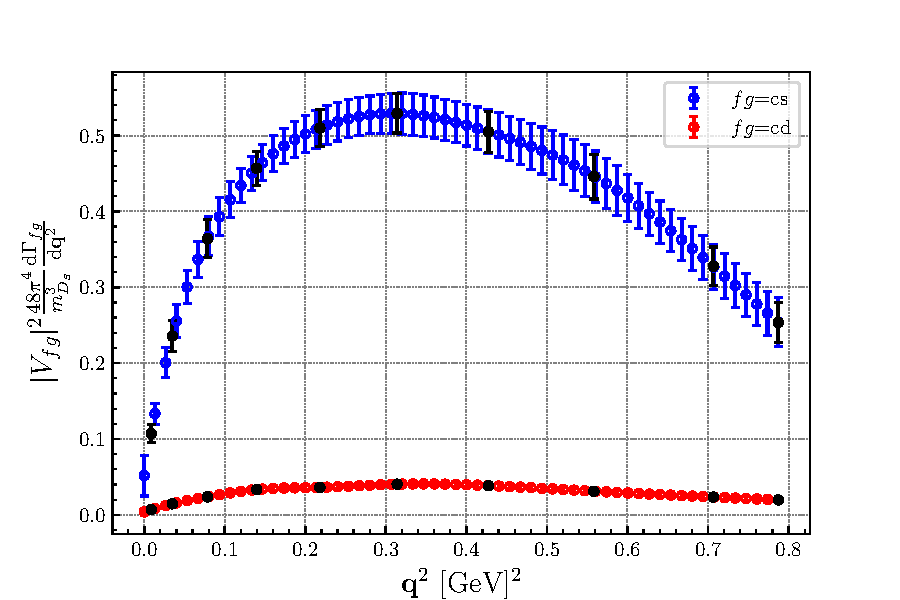
\includegraphics[scale=0.8]{plots/final_DgammaDq2.pdf}
  \caption{Preliminary values of the differential decay rate of
  $D_s\to X\ell\bar\nu$.
  the contribution form the $cd$ channel (in red) is observed to be smaller than
  the contribution form the $cd$ channel and (in blue) mainly due to $V_{cs}>V_{cd}$.}
  \label{fig:dGammadq_Ds}
\end{figure}


\subsection{Sub-project 2: Bottom quark mass $m_b$}
\label{sec:mb}

In this sub-project we describe the determination of the $b$-quark
mass. We can extract the mass of the $B$ and $B_s$ pseudo-scalar mesons ($M_{B}$ and $M_{B_s}$)
from the right diagram of Figure~\ref{fig:4pt} representing the two-point function
\begin{equation}
  \langle B_{(s)}(\bm{0},t) B_{(s)}^\dagger({\bf 0},0)\rangle\xrightarrow{t>>a, (T-t)>>a}
  \frac{1}{2M_{B_{(s)}}}|\langle 0 | B_{(s)} | B_{(s)}\rangle|^2\left(e^{-M_{B_{(s)}} t}+e^{-M_{B_{(s)}}(T-t)}\right)
  \,
  \label{eq:Mb}
\end{equation}
with the operators
\[
B({\bf 0},t)=\frac{1}{L^3}\sum_{\bf x}\bar b\gamma_5 u({\bf x},t)\,,\qquad
B_s({\bf 0},t)=\frac{1}{L^3}\sum_{\bf x}\bar b\gamma_5 s({\bf x},t)\,.
\]
In quantities involving a (valence) $b$-quark, we expect lattice
artefacts of the order $(am_b)^2$, which can be significant even with
the lattice spacing values employed in this project. Therefore, it is
advisable not to work directly at the $b$-quark mass, but to apply the
ratio method: The $b$-quark mass is obtained as an interpolation
between quark masses in the charm region and the static limit.
Thus, we compute Eq.~(\ref{eq:Mb}) replacing the $b$ quark with six heavy quarks $h$
in the range of $m_h\in [m_c,3.5m_c]$
and for each we compute the ratio
\begin{equation}
  Q_m = \frac{M_{hs}}{M_{h\ell}^\gamma M_{cs}^{(1-\gamma)}}\,,
  \label{eq:ratio_Q}
\end{equation}
where $M_{hs}$ and $M_{hl}$ are the heavy-strange and heavy-light
pseudo-scalar masses, respectively, while we denote by $M_{cs}$
the mass of the pseudo-scalar meson made out of a charm
and a strange quark. The parameter $\gamma$ is a free parameter in the range $[0, 1)$.
The asymptotic behaviour of $Q_m$ can be computed using HQET reading
\begin{equation}
  \lim_{ m^{pole}_h\to \infty}
  \frac{M_{hs}}{( m^{pole}_h)^{(1-\gamma)} M_{h\ell}^\gamma}=\mbox{const.}\,,
  \label{eq:yHQFTlim}
\end{equation}
where $ m^{pole}_h$ is the pole mass of the heavy quark.
We then consider a sequence of heavy quark masses such that any two
successive masses have a common and fixed ratio i.e.
$ m_h^{(n)}=\lambda m_h^{(n-1)}, n=2,3,...$ and we construct the
following ratios at given lattice spacing $a$
\begin{equation}
  \begin{split}
    y_Q( m^{(n)}_h,a)&=\frac{Q_m( m_h^{(n)},a)}{Q_m( m_h^{(n-1)},a)}\cdot
    \left(\frac{ m_{h}^{(n)} \rho( m_{h}^{(n)})}{ m_{h}^{(n-1)}\rho( m_{h}^{(n-1)})}\right)^{(\gamma-1)}\\
    &=\lambda^{(\gamma-1)}\frac{Q_m( m_h^{(n)},a)}{Q_m( m_h^{(n-1)},a)}\cdot
    \left(\frac{ \rho( m_{h}^{(n)})}{\rho(
      m_{h}^{(n-1)})}\right)^{(\gamma-1)}\\\,,
  \end{split}
\end{equation}
where we have used the relation  $ m^{pole}_h= m_{h}^{} \rho( m_{h}^{})$
between the $\overline{\mbox{MS}}$ renormalised mass and the pole
mass, which is known perturbatively up to N$^3$LO~\cite{Chetyrkin:1999pq}.
For each pair of heavy quark masses, we carry out a continuum
extrapolation separately
\footnote{We do not need a chiral extrapolation since we are already at physical point.}
obtaining $y_Q( m^{(n)}_h)=y_Q( m^{(n)}_h,a=0)$.
In the continuum limit, the ratios $y_Q( m^{(n)}_h)$ can be described
in terms of the heavy mass $m_h$ as~\cite{ETM:2011zey}
\begin{equation}
  y_Q( m^{(n)}_h) = 1 + \frac{\eta_1}{ m_h}+ \frac{\eta_2}{ m_h^2}\,,
  \label{eq:fity}
\end{equation}
where $\eta_{1,2}$ are free parameters and the limit in
Eq.~(\ref{eq:yHQFTlim}) has already been taken into account.
Finally, the $b$-quark mass can be computed with
\begin{equation}
  y_Q( m^{(2)}_h)y_Q( m^{(3)}_h)...y_Q( m^{(K+1)}_h)\frac{Q_m( m_h^{(1)},a)}{\lambda^{K(\gamma-1)}}
  \left(\frac{ \rho( m_{h}^{(K+1)})}{\rho( m_{h}^{(1)})}\right)^{(1-\gamma)}=Q_m( m_h^{(K+1)},a)
  \,,
\end{equation}
where the ratios $y_Q$ on the left-hand-side are evaluated using the
fit function Eq.~(\ref{eq:fity}) and the parameters $\lambda$, $K$ and
$ m_h^1$ chosen such that $Q_m( m_h^{(K+1)},a)$ matches 
the experimental value of the ratio $M_{B_s}/(M_{B}^\gamma M_{D_s}^{(1-\gamma)})$.


\endinput

% %\textit{Describe your research project in detail, structured in sub-projects, if applicable. Include discussion of the scientific questions that you are planning to address and the overall scientific goals of the project. It is important that you describe the innovative aspects, impact and topicality of the proposal.}
% %\begin{itshape}
% %\begin{itemize}\setlength{\itemsep}{-2pt}
% %  \item Scientific questions you want to address
% %  \item Scientific objectives
% %  \item Computational objectives
% %  \item Approach and expected outcome
% %  \item Expected impact on the research area
% %  \item Scientific and technical innovation potential, impact and topicality
% %  \item Progress beyond the state-of-the-art
% %\end{itemize}
% %\end{itshape}
% %
% %\subsubsection{Sub-project 1}
% %\subsubsection{Sub-project 2}
% %\textit{...}\\


\subsection{Review Processes}

Here we list the projects that are closely connected to the present
proposal and which are funded through third party grants.

\textbf{C. Urbach:} \textit{NuMeriQS}, DFG funded Collaborative research center CRC1639\footnote{\protect\url{https://numeriqs.hiskp.uni-bonn.de}}.

\section{Numerical Methods and Algorithms} 
 

\label{sec:algos}
\rule{\textwidth}{0.4pt}\\

As discussed in Section~\ref{sec:proj} the major computational effort is 
the evaluation of the four-point function \eqref{eq:4pt} by computing the
contractions depicted in Fig.~\ref{fig:4pt}.
We propose to compute those using stochastic time-slice sources with
spin dilution at $t_{src}$ with a sequential inversion through the
sink $B_s$-meson vertex at $t_{snk}$ and a second sequential inversion
at $t_2$ with the weak current and a momentum injection ${\bf q}$.
The sequential inversions are labelled with a semicircular arrow next to
the vertices in Fig.~\ref{fig:4pt}. We plan to have five values of the
momenta to cover all the physical region.

In order to isolate the ground state, the two currents in the
four-point function of Fig.~\ref{fig:4pt} should be well separated
from the $B_s$-meson interpolating field. However, the exponential
deterioration of the signal-to-noise ratio as a function of Euclidean
time, long time understood in terms of the Parisi-Lepage framework,
poses a serious limitation. To overcome this limitation we employ
Jacobi smearing for the quark fields of the $B_s$
operator~\cite{Allton:1993wc}, combined with APE smearing of the gauge
links~\cite{FALCIONI1985624} used in the Jacobi smearing kernel.  
The usage of the smearing allows us to reach ground state dominance 
with a shorter time separation of source and sink compared to without
smearing. This is shown in Fig.~\ref{fig:smearing}, where the
effective mass of the $D_s$ meson
\begin{equation}\label{eq:meff}
	M_{eff}^{D_s}(t)\ =\ \ln\frac{C(t)}{C(t+1)}	
\end{equation}
is shown in lattice units as a function of the source sink separation $t=t_{snk}-t_{src}$. We compare the effective mass
computed from a local-local correlation function with the one computed from
a smeared-smeared correlation function (blue circles). Ground state
dominance is reached significantly earlier for the smeared correlation
function. 
             
\begin{SCfigure}[0.5]
  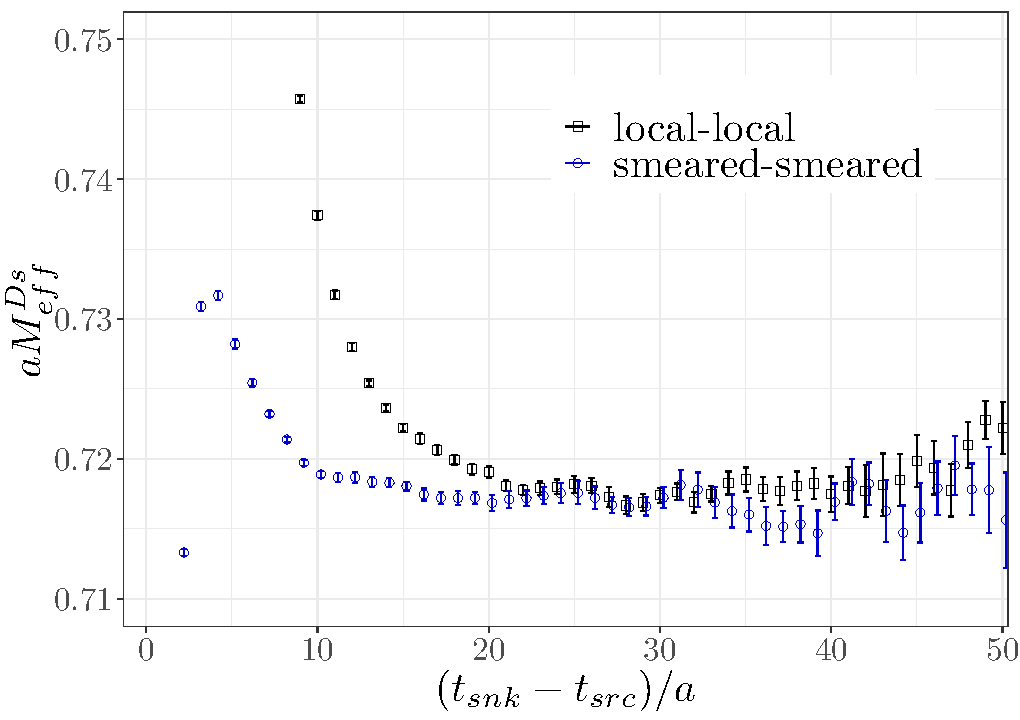
\includegraphics[width=0.59\textwidth]{plots/smearing_MDs.pdf}
  \caption{Comparison of the effective mass \eqref{eq:meff} of the correlator
    \eqref{eq:2pt}  computed with
    smeared quark field (smeared-smeared) and unsmeared (local-local)} 
  \label{fig:smearing}
\end{SCfigure}

For the contraction of the quark loops we will use nissa software
suite\footnote{nissa is public available at
\url{https://github.com/sunpho84/nissa}}, a C++  software for lattice
QCD calculations. The package provides the functionality for memory
distributed and shared memory systems and it supports all contractions 
needed for this proposal.

\subsection{The multi-grid solver}
The algorithms and codes to be used for this project are developed  for the NVIDIA GPU architecture
and thus are very well suited for the JUWELS booster module. For the solver we will use the QUDA library~\cite{Clark:2009wm,Babich:2011np,Clark:2016rdz} which provides optimised kernels for NVIDIA GPUs.
Simulations close to or at the physical point, like in this project, are  expensive, with the most computationally demanding component being the generation of quark propagators that require to invert the Dirac operator.

We will employ the state-of-the-art QUDA multigrid (MG) solver, a MG-preconditioned generalised conjugate residual (GCR) which has been further improved through the introduction of coarse-grid deflation.
Because we will employ twisted boundary conditions~\cite{deDivitiis:2004kq} to access arbitrary momentum configurations, we need to rerun the MG setup once for each phase angle.
As a result we will not make use of the coarse-grid deflated variant of the solver since the setup cost would then exceed the cost of the inversions for this particular project.
Still, the resulting solver is in a single solve much faster than the highly optimised implementation of the mixed-precision conjugate gradient (CG) algorithm in QUDA.
This is illustrated in \Cref{fig:multi-grid}, where we compare the time to solution between MG and mixed-precision CG for a range of valence quark masses ranging from the charm quark mass to the physical light quark mass.
The results obtained on a $64^3 \cdot 128$ lattice on eight JUWELS Booster nodes indicate that at the physical light quark mass, MG is more than 200 times faster than CG.
The disadvantage of MG solvers, however, is that they strong scale poorly due to the significantly smaller coarse grid system.

\begin{SCfigure}[0.5]
	\includegraphics[width=0.59\textwidth]{./plots/mg_vs_cg.pdf}
	\caption{Comparison between the time to solution for inverting the
    twisted mass clover Dirac matrix for one right-hand-side using
    the fastest mixed-precision CG in QUDA at different quark masses 
    against a tuned MG-preconditioned GCR on a $64^3\cdot128$ lattice
    on 8 nodes on JUWELS Booster. The dashed vertical lines indicate the
    approximate physical light ($\mu_{u,d}$), strange ($\mu_s$) and
    charm ($\mu_c$) quark masses.}
	\label{fig:multi-grid}
\end{SCfigure}

%% \textbf{Method}
%% \begin{itemize}
%%   \item depends on walltime, time-to-solution, time for contractions (plegma, quda )
%%     %%%
%%   \item low-mode deflation + hierarchical probing with 3 random vectors
%%     %%%
%%   \item volume sources ($\mathcal{O}(1000)$)
%%     %%%
%%   \item spin, color, time dilution ?
%%     %%%
%%   \item ``Frequency-splitting estimators of single-propagator traces'' ?
%%     %%%
%%   \item strange / charm loops ? OS / unitary ?
%% \end{itemize}

%\textbf{Misc}
%\begin{itemize}
%  \item meson-meson / baryon-baryon 2pt functions to build disc. contributions to ffs ? \\
%    \textbf{In case of renewal application:} do we have enough connected parts to demonstrate physics results / impa%ct of disc ?
%    %%%
%  \item smearing
%\end{itemize}


\endinput



\section{Computer Resources}

\subsection{Code Performance and Workflow}

%\begin{SCtable}[1.]
%  \centering % center the table
%  \begin{tabular}{crrr} % alignment of each column data
%    \toprule
%    $V$ & $N$ & $t/s$ per solve & speedup\\
%    \midrule
%    $64^3\times128$ & 8 & 3.60 & 1\\
%    & 16 & 2.04 & 1.76\\
%    \midrule
%    $80^3\times160$ & 20 & 2.75  & 1\\
%    & 40 & 1.59 & 1.72\\
%    \bottomrule
%  \end{tabular}
%  \caption{Timings for QUDA MG solves on NVIDIA's Selene supercomputer
%  for one configuration of ensemble cB211.072.64 and one of ensemble
%  cC211.06.80 with $N$ the number of GPUs.}
%  \label{tab:MGsolver}
%\end{SCtable}


%All performance results have been measured on JUWELS Booster
About 90\% of the total run-time in the different parts of our research proposal is spent in QUDA's MG solver, the scaling behavior of which depends on the performance of the fine-grid Dirac operator ($D$) in double and single precision, as well as the intermediate-grid ($D_c$) and coarse-grid ($D_{cc}$) Dirac operators in half precision, which all have slightly different scaling behaviors due to the amount of parallelism that can be exposed on each grid.
On many nodes, only a small part of the solver time is spent in other kernels such as linear algebra.
Because the MG algorithm has substantial device memory requirements, it cannot be run as a whole on few GPUs and then scaled to many GPUs.
Similarly, it cannot be weak-scaled using synthetic data as the amount of time spent in each kernel depends on the physical properties of the Dirac operator to be inverted (and the associated gauge field).
Therefore, we demonstrate scalability via
\begin{itemize}
	\item  a combination of micro-benchmarks of the individual kernels depicted in \Cref{fig:quda_dirac_strong},
	\item time-to-solution of the multigrid solver in \Cref{tab:MGsolver},
	\item and a comparison of the time-to-solution obtained on various HPC systems equipped with NVIDIA GPUs  in \Cref{fig:multigrid_comparison}.
\end{itemize}
As depicted in \Cref{fig:quda_dirac_strong}, the scaling of the kernels involving the full-sized problem is close ideal up to a large number of nodes.
Only the coarse-grid Dirac operators, $D_c$ and $D_{cc}$, do not show a good scaling due to the significantly reduced problem size.
The multigrid solver is the only component affected by it and its scaling is sub-optimal due to the fact that most of the time is spent on the coarse-grid kernels. For this reason we use in our calculations the smallest number of nodes where our full problem can fit and run in parallel multiple jobs on different configurations.
The nodes we will used are reported in Table~\ref{tab:MGsolver}, respect to the
previous stage of this project we manage to optimize the memory footprint
of our run such that we can run in half of the nodes for the ensembles cB211.072.64
and cC211.06.80 resulting in more efficient runs.
In our runs the majority of the time will be spend in the setup of the MG
which will only be necessary for the first inversion for each values of the momentum.
%We will use 8 nodes for the cB211.072.64 ensemble, 24 nodes for the  , 20 nodes for the cC211.06.90 ensemble
%and 96 for the cD211.054.96 ensemble.

\begin{SCfigure}[0.5]
	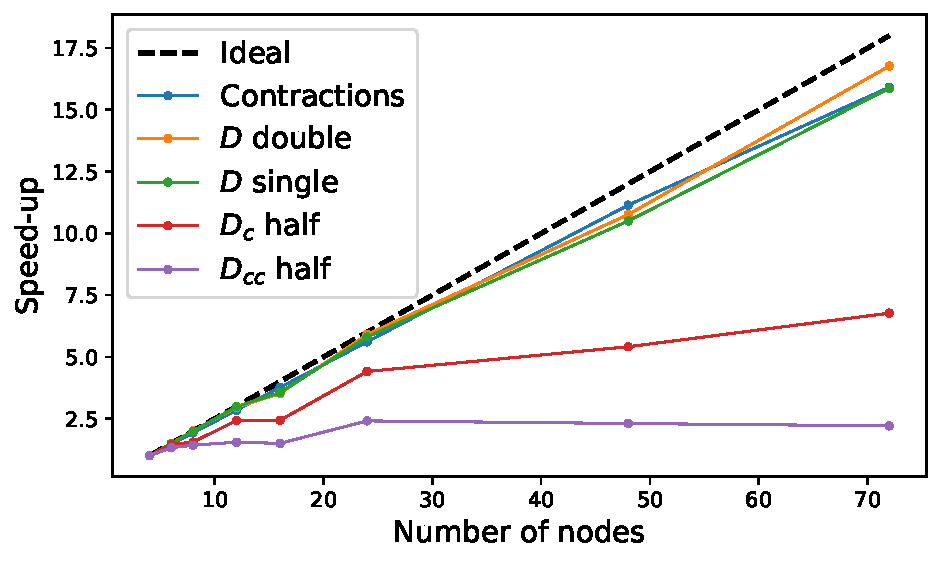
\includegraphics[width=0.6\textwidth]{plots/speedup.pdf}
	\caption{Strong scaling study of the contraction kernels and the QUDA Dirac operators on the fine ($D$), intermediate ($D_c$) and coarse ($D_{cc}$) grids for the cD211.054.96 having a lattice of size $96^3\times128$.}
	\label{fig:quda_dirac_strong}
\end{SCfigure}

\begin{table}%[1.]
	\centering % center the table
	\begin{tabular}{cccccccc} % alignment of each column data
		\toprule
		Ensemble      & $V$             & $N$ & $t/s$ MG setup & $t/s$ MG update & \multicolumn{3}{c}{$t/s$ MG inversion}                         \\
		              &                 &     &                &                 & $\ell$-quark                           & $s$-quark & $h$-quark \\
		%		\midrule
		\midrule
		% cAp211.077.64 & $64^3\times128$ & 8  & 52.6 & 0.5  & 2.6  & 0.8 & 0.3\\
		\midrule
		cB211.072.48  & $48^3\times96$  & 2   & 35.7           & 0.7             & 0.7                                    & 0.9       & 0.7       \\
		cB211.072.64  & $64^3\times128$ & 4   & 87.5           & 0.9             & 3.3                                    & 1.3       & 1.0       \\
		% cB211.072.64  & $64^3\times128$ & 8   & 51.5           & 0.5             & 2.6                                    & 0.8       & 0.3       \\
		cB211.072.96  & $96^3\times192$ & 24  & 57.9           & 1.0             & 4.15                                   & 1.1       & 1.1       \\
		\midrule
		% cC211.06.80   & $80^3\times160$ & 20  & 36.5           & 0.6             & 1.9                                    & 0.8       & 0.8       \\
		cC211.06.80   & $80^3\times160$ & 10  & 62.9           & 1.0             & 2.7                                    & 1.1       & 1.2       \\
		%		\midrule
		% cC211.06.112 & $112^3\times224$ & 56 & 43.6 & 0.9 & 2.87 & 1.0 & 0.5 \\
		\midrule
		cD211.054.96  & $96^3\times192$ & 24  & 46.0           & 1.0             & 2.5                                    & 1.0       & 1.2       \\
		\midrule
		cE211.044.112 & $112\times224$  & 56  & 43.6           & 1.0             & 2.87                                   & 1.0       & 1.3      \\
		\bottomrule   &
	\end{tabular}
	\caption{Timings for QUDA solves the ensembles we will use in this project.
		The light ($\ell$) and strange ($s$) quarks are inverted using the MG solver.
		The heavy ($h$) quark is inverted using the CG solver.
	}
	\label{tab:MGsolver}
\end{table}

\begin{SCfigure}[0.5]
	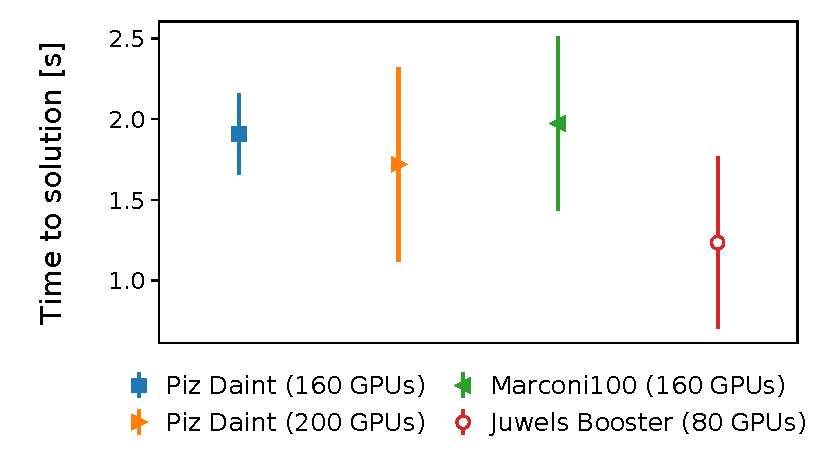
\includegraphics[width=0.6\textwidth]{plots/comparison.pdf}
	\caption{Comparison of the time to solution of the multigrid solver for the cC211.06.80 ensemble on different HPC systems in Europe and number of nodes.}
	\label{fig:multigrid_comparison}
\end{SCfigure}

Furthermore, in \Cref{fig:multigrid_comparison} we show a comparison of the time-to-solution for the cC211.06.80 ensemble measured on various
HPC systems in Europe equipped with different models of NVIDIA GPUs. We show results obtained on Piz Daint at CSCS equipped with P100, on Marconi100 at Cineca equipped with V100 and on the JUWELS Booster equipped with A100. The latter shows a time-to-solution about 40\% than the other systems using half of the GPUs. This is thanks to the improved performance of the latest model but also thanks to the significantly larger device memory available. Therefore our application has a significant speed-up on the GPU architecture offered by the JUWELS Booster.


\endinput





We justify our requested resources for the goals described
in \Cref{sec:proj} in the table below.

\subsubsection{Run types \label{sec:runtypes}}

For each ensemble we plan to compute the four-point function of Fig.~\ref{fig:4pt} in the followign way: we start computing the quark propagator of the spectator $u$ and $s$, this requires
one MG setup for the $u$ and then un update for the strange.
Then we compute the heavy quark propagators, one direct and two sequential (on the $u$ and $s$ propagators), for each heavy of the six heavy quark masses ($m_h=n m_c$ with $n=1, 1.5, 2, 2.5, 3, 3.5$). For each quark mass we need an update of the MG.
The two sequential propagator produced so far, with 4 insertions of the axial ($\gamma_5\gamma_\mu$ with $\mu=0,1,2,3$) and 4 insertions of the vector current ($\gamma_\mu$), will be used as a source for a further inversion of the light $\ell$- and $c$-quark, this requires one MG setup due to the different value of the momenta used and one update to pass from the $\ell$- to the $c$-quark, the setup can be reused within the inversions with the same momentum.

% For each ensemble, we plan to compute  one quark propagator for the strange
% and five for the heavy quark ($m_h=n m_c$ with $n=1, 1.5, 2, 2.5, 3, 3.5$) all at zero momentum, the strange and the heavy propagator 
% will be computed with the MG solver, thus one setup of the MG is needed and then one update for each 
% heavy quark. 
% The source used will be a stochastic smeared source.
% Then we compute the sequential propagator necessary to build the four-point function in Fig.~\ref{fig:4pt},
% first inverting the list of heavy Dirac operators using as source strange propagator with a pseudo-scalar
% insertion and smeared. Then the resulting vectors will be used as a source for a further inversion of the light u-quark and for the c-quark for 10 values of momenta with the 4 insertions of the axial ($\gamma_5\gamma_\mu$ with $\mu=0,1,2,3$) and 4 insertions of the vector current ($\gamma_\mu$). The last set of sequential inversions (u-quark of Fig.~\ref{fig:4pt} and the equivalent substituting the u-quark with a c-quark) require one MG setup due to the different value of the momenta used, but the setup can be reused for all the inversions with the same momentum.
% In addition, for creating the two-point function in Fig.~\ref{fig:4pt} for the $B$ meson (necessary to construct the ration of Eq.~\ref{eq:ratio_Q}) one
% inversion for the light quark with zero momentum is necessary, in this case, the MG setup can be then reused for the strange quark inversion.
All the previous sets of inversion will be repeated 4 times due to the spin dilution
and for a series of stochastic sources listed below reusing the same MG setup. 
however to repeat the inversions for the 10 values of the momenta we plan to use and 
for different gauge configurations a new MG setup will be constructed.
The number of stochastic sources is scaled with the volume to keep the error of the different ensembles constant. We measured that the smearing and the contraction time account for 15\% of our running time and we added it to the cost.

In the table below we refer to the following types of runs:
\begin{enumerate}
	% \item \label{rt:cAp64} 10 stochastic sources for the cAp211.077.64
	\item \label{rt:cB48} 10 stochastic sources for 300 gauge configurations for the cB211.072.48
	\item \label{rt:cB64} 5 stochastic sources for 300 gauge configurations the cB211.072.64
	\item \label{rt:cB96} 3 stochastic sources for 300 gauge configurations the cB211.072.96
	\item \label{rt:cC80} 3 stochastic sources for 300 gauge configurations the cC211.06.80
	      % \item \label{rt:cC112} 2 stochastic sources for the cC211.06.112	
	\item \label{rt:cD96}  3 stochastic sources 300 gauge configurations for the cD211.054.96
	\item  \label{rt:cE112} 2 stochastic sources 300 gauge configurations for the cE211.044.112
\end{enumerate}
We plan to have a job for each configuration and each value of the momentum, then
all the stochastic sources will be processed in the same job run.

\begin{center}
	{\small
		\begin{tabular}{lllccccr} \hline\hline
			Sub-         &
			Type         &
			Problem      &
			\# runs      &
			\# steps/    &
			Wall time/   &
			\# cores/    &
			Total                                                                                                               \\
			project      &
			of run       &
			size         &
			             &
			run          &
			step [hours] &
			run          &
			[core-h]                                                                                                            \\
			\hline\hline
			%%%%
			%%%%
			%%%%
			% 1-2          & (\ref{rt:cAp64}) & $64^3\times 128$  & $10\times 400$ & 1 & 1.63 & 8 nodes  & $2.5 \times 10^6$       \\
			1-2          & (\ref{rt:cB48})  & $48^3\times 96$  & $10\times 300$ & 1 & 2.2  & 2 nodes  & $0.6 \times 10^6$      \\
			             & (\ref{rt:cB64})  & $64^3\times 128$  & $10\times 300$ & 1 & 1.6 & 4 nodes  & $1.0 \times 10^6$      \\
			             & (\ref{rt:cB96})  & $96^3\times 192$  & $10\times 300$ & 1 & .97 & 24 nodes & $3.3 \times 10^6$      \\
			             & (\ref{rt:cC80})  & $80^3\times 160$  & $10\times 300$ & 1 & 1.1 & 10 nodes & $1.6 \times 10^6$      \\
			%  & (\ref{rt:cC112}) & $112^3\times 224$ & $10\times 400$ & 1 & 0.32 & 56 nodes & $3.4 \times 10^6$       \\
			             & (\ref{rt:cD96})  & $96^3\times 192$  & $10\times 300$ & 1 & 0.95 & 24 nodes & $3.3 \times 10^6$      \\
			             & (\ref{rt:cE112}) & $112^3\times 224$ & $10\times 300$ & 1 & 0.68 & 56 nodes & $5.5 \times 10^6$      \\
			%multyply by 10/9 for smearing and contractions 			
			%%%
			%%%
			%%%
			\hline\hline
			TOTAL        &                  &                   &                &   &      &          & $15.3\times 10^6$ core-h \\
		\end{tabular}
	}
\end{center}
\bigskip
We thus ask for a total amount of \textbf{15.3 Mcore-h}, equivalent to \textbf{91983 EFLOP}\footnote{conversion factor 6012 EFLOP / Mcore-h}  on the \textbf{JUWELS-Booster} module at JSC.
%%% \textit{(0.5 to 1 page)}



\section{Resource Management and Work Schedule}
\rule{\textwidth}{0.4pt}
\subsection{Resource management}

Our team has extensive experience in managing large computer time
allocations, having been awarded two PRACE Tier-0 allocations, many
NIC Gauss computing allocations, large scale production projects on
JUWELS Booster, Marconi100 at Cineca and Piz Daint at CSCS in
Switzerland, and a number of smaller local computer time
allocations. These allocations exceed 500 Mi core-hours in total. The
team will follow established practices for monitoring resources and
progress, including periodically (around once a week) telephone
conferences and local group meetings.  During these calls adherence to
the schedule proposed below will be evaluated, with corrections made
if necessary.

\subsection{Work schedule}

\begin{figure}[tbp]
  \begin{ganttchart}[
      x unit=0.335cm,        
      y unit title=0.5cm,
      y unit chart=0.5cm,
      vgrid,hgrid,
      %        title label anchor/.style={below=-1.6ex},
      bar label font=\small,
      title left shift=.05,
      title right shift=-.05,
      title height=1,
      incomplete/.style={fill=white},
      progress label text={},
      bar height=0.8,
      bar top shift=+0.1,
      group right shift=0,
      group top shift=.0,
      group height=.0
    ]{1}{48}
    %labels
    \sffamily
    \gantttitle{\textbf{Allocation duration}}{48} \\
    \gantttitle{Nov.}{4} 
    \gantttitle{Dec.}{4} 
    \gantttitle{Jan.}{4} 
    \gantttitle{Feb.}{4} 
    \gantttitle{Mar.}{4} 
    \gantttitle{Apr.}{4}
    \gantttitle{May.}{4} 
    \gantttitle{Jun.}{4} 
    \gantttitle{Jul.}{4} 
    \gantttitle{Aug.}{4} 
    \gantttitle{Sep.}{4} 
    \gantttitle{Oct.}{4}
    \\
\ganttbar[inline,bar/.style={fill=blue!30}]{cB64}{1}{8}\\
\ganttbar[inline,bar/.style={fill=blue!60}]{cB96}{8}{14}
\ganttbar[inline,bar/.style={fill=green!30}]{cC80 }{15}{24}
\ganttbar[inline,bar/.style={fill=magenta!30}]{cD96 }{24}{30}\\
\ganttbar[inline,bar/.style={fill=green!60}]{cC112 }{30}{40}
\ganttbar[inline,bar/.style={fill=red!30}]{cAp64 }{41}{48}
%    \gantttitle{Sub-project 1: pion and kaon $\langle x^n\rangle$}{48}\\
%    \ganttbar[inline,bar/.style={fill=red!30}]{cB64 connected 2- and 3-pt}{1}{48}\\
%    \ganttbar[inline,bar/.style={fill=blue!20}]{cB64 light/strange loops}{1}{48}\\
%    
%    \gantttitle{Sub-project 2: hadronic vacuum polarisation}{48}\\
%    \ganttbar[inline,bar/.style={fill=red!20}]{cC112 meson 2pt functions}{1}{48}\\
%    \ganttbar[inline,bar/.style={fill=blue!20}]{cB48 meson 2pt functions}{1}{16}
%    
  \end{ganttchart}
  \caption{A Gantt chart describing the scheduling of the steps
    involved in our calculation.}
  \label{fig:gantt}
\end{figure}

Since we are dealing in this proposal only with the estimation of
observables on already existing gauge configurations, all separate
runs are independent and, thus, runs for different configurations do
not depend on each other. We will avoid to store so-called propagators
completely, all contractions will be performed on the fly.

We plan to run all tasks sequentially as indicated in the Gantt
chart \Cref{fig:gantt}. 

\endinput



\section{Key Personnel and Experiences}
\rule{\textwidth}{0.4pt}\\
\\
The proposers have extensive and long standing experience in high
performance computing using vector and massively parallel
supercomputers such as the CRAY T3E, PC-Cluster systems, APE, IBM
Blue Gene, Intel Xeon Scalable and Intel Knight's Landing machines as well
as machines equipped with GPU-based accelerators.
Our group includes algorithm experts who have been involved over many years in
developing efficient implementations of dynamical fermion algorithms.

\noindent\textbf{Carsten Urbach (PI)} is professor at the University
of Bonn. He has pioneered simulation methods in lattice QCD applying
mass preconditioning and multiple timescale integration schemes and
flavour singlet calculations. He is and has been managing Gauss
project allocations at JSC and LRZ and he is principal investigator in
two DFG funded collaborative research centres.\\
\noindent\textbf{Roberto Frezzotti} is professor of physics at the
University of Rome II. He is one of the fathers of Wilson twisted mass
lattice QCD and the key feature of automatic improvement at maximal
twist.\\ 
\noindent\textbf{Nazario Tantalo} is professor of physics at the
University of Rome II. He is one of the developers of the spectral
reconstruction method, which is key to this proposal.

\section{Bibliographic References}

\footnotesize{
	\bibliography{bibliography}
}

\end{document}
